\documentclass[aps,pra,twocolumn,reprint,floatfix,amsmath,amssymb]{revtex4-2}

\usepackage{graphicx}
\usepackage{booktabs}
\usepackage{siunitx}
\usepackage[colorlinks=true,linkcolor=blue,citecolor=blue,urlcolor=blue,hypertexnames=false]{hyperref}
\usepackage{float}
\usepackage{xcolor}
\usepackage{array}

\newcommand{\ket}[1]{\lvert #1 \rangle}
\newcommand{\bra}[1]{\langle #1 \rvert}
\newcommand{\avg}[1]{\langle #1 \rangle}
\newcommand{\dd}{\mathrm{d}}

\begin{document}

\title{Sequential Active Cooling of a Storage Cavity Through a Transmon-\(f\) Ladder}
\author{Execution Engineer}
\date{\today}

\begin{abstract}
This study evaluates whether the local circuit-QED device model can support an experimentally useful storage-cooling primitive based on the ladder \(\ket{g,0_r,n_s}\rightarrow\ket{f,0_r,n_s-1}\rightarrow\ket{g,1_r,n_s-1}\rightarrow\ket{g,0_r,n_s-1}\) for \(n_s=1,\ldots,4\). The analysis uses the editable local three-mode transmon-storage-readout model already present in the simulation environment and treats the relevant storage and readout sidebands as effective activated interactions. Guided by the sideband-control literature, especially Ref.~\onlinecite{huang2025fastsideband}, the study combines dressed-state spectroscopy, pulse-family scans, qualitative Floquet checks, and open-system cooling simulations. The Step A frequencies \(\ket{g,0_r,n_s}\leftrightarrow\ket{f,0_r,n_s-1}\) are \(6.804115034\), \(6.798434192\), \(6.792753350\), and \(6.787072508~\si{\giga\hertz}\); the Step B frequencies \(\ket{f,0_r,n_s-1}\leftrightarrow\ket{g,1_r,n_s-1}\) are \(3.448825278\), \(3.443144436\), \(3.437463594\), and \(3.431782752~\si{\giga\hertz}\). Adjacent \(n_s\)-resolved lines are separated by only \(5.680842~\si{\mega\hertz}\), so pulse bandwidth rather than large spectral gaps sets selectivity. Paper-motivated smooth bump ramps are the best Step A family for three of the four storage manifolds, while a cosine-squared pulse is the best Step B family for all \(n_s\). The resulting single-cycle cooling success ranges from \(96.20\%\) to \(97.35\%\), and a four-step ladder starting from \(\ket{g,0_r,4}\) lowers the mean storage occupation to \(0.0757\). The main caveat is explicit: the present model validates effective-control feasibility and calibration strategy, but it does not derive the sideband rate or Stark shift from a microscopic pump Hamiltonian.
\end{abstract}

\maketitle

\section{Introduction}
Fast sideband control has emerged as a compelling route to bosonic-mode manipulation in weakly dispersive circuit-QED hardware because it can amplify interaction rates beyond the bare dispersive scale while preserving photon-number resolution~\cite{blais2021circuit,huang2025fastsideband}. Reference~\onlinecite{huang2025fastsideband} is especially relevant to the present device problem: it emphasizes charge-driven sideband activation, photon-number-resolved spectroscopy and calibration, bosonic enhancement of exchange rates, strong-drive Stark and Floquet effects, and the practical value of smooth ramps over naive square pulses.

The present target is not the same protocol as Ref.~\onlinecite{huang2025fastsideband}. Instead of state preparation or unitary SWAP synthesis within a multimode memory, the objective here is a dissipative cooling primitive for the storage cavity,
\begin{equation}
\begin{aligned}
\ket{g,0_r,n_s} &\rightarrow \ket{f,0_r,n_s-1} \\
&\rightarrow \ket{g,1_r,n_s-1}
\rightarrow \ket{g,0_r,n_s-1},
\end{aligned}
\label{eq:cooling_cycle}
\end{equation}
for \(n_s=1,\ldots,4\). The first step converts one storage photon into transmon \(f\)-manifold excitation, the second transfers that excitation into the lossy readout mode, and the third uses readout decay to make the map irreversible.

The study therefore asks nine concrete questions. Can the ladder of Eq.~\eqref{eq:cooling_cycle} be realized in the local device? What are the dressed frequencies for each \(n_s\)? Which physical mechanism best activates the two coherent steps? Which pulse families are most selective? Do strong-drive Stark shifts or Floquet effects alter the calibration strategy? Does the full sequence cool rather than merely reshuffle excitation coherently? What are the dominant leakage channels? How should the protocol be validated experimentally? And which uncertainties remain after the present simulation pass?

The report is organized as follows. Section~\ref{sec:system} defines the basis conventions, Hamiltonian, and connection to the sideband literature. Section~\ref{sec:results} presents dressed spectroscopy, pulse-design results, and dissipative cooling performance. Section~\ref{sec:validation} checks analytic consistency, numerical convergence, and literature alignment. Section~\ref{sec:discussion} translates the results into experiment-facing guidance. Section~\ref{sec:future} records the main limitations and the next steps. Detailed tables, validation plots, and reproducibility information appear in the appendices.

\section{System and Methods}
\label{sec:system}

\subsection{Basis, Units, and Device Parameters}
Throughout this report the basis ordering is
\begin{equation}
\ket{q,n_r,n_s},
\label{eq:basis_definition}
\end{equation}
where \(q\in\{g,e,f,\ldots\}\) is the transmon state, \(n_r\) is the readout occupation, and \(n_s\) is the storage occupation. This is the user-facing convention required for the study. Internally, the simulator stores the tensor factors in the order transmon, storage, readout; all exported labels are permuted into Eq.~\eqref{eq:basis_definition} before analysis and reporting.

Internal simulator frequencies are angular frequencies in \(\si{\radian\per\second}\), while times are in \(\si{\second}\). All quoted frequencies in the text and tables are converted into ordinary frequencies in \(\si{\hertz}\), \(\si{\mega\hertz}\), or \(\si{\giga\hertz}\). The default rotating frame subtracts the bare transmon, storage, and readout frequencies.

The local device model is the three-mode dispersive Hamiltonian
\begin{equation}
\begin{split}
\frac{H_0}{\hbar}={}&
\omega_q \hat{n}_q
+ \frac{\alpha}{2}\hat{n}_q(\hat{n}_q-1)
+ \omega_s \hat{n}_s
+ \omega_r \hat{n}_r \\
&+ \chi_s \hat{n}_q \hat{n}_s
+ \chi_r \hat{n}_q \hat{n}_r
+ \chi_{sr}\hat{n}_s \hat{n}_r \\
&+ \frac{K_s}{2}\hat{n}_s(\hat{n}_s-1)
+ \frac{K_r}{2}\hat{n}_r(\hat{n}_r-1),
\end{split}
\label{eq:drift}
\end{equation}
with the parameter values listed in Table~\ref{tab:device_parameters}. The important sign conventions are \(\alpha<0\), \(\chi_s<0\), and \(\chi_r<0\). In the present device configuration, \(\chi_{sr}=K_s=K_r=0\).

\begin{table}[t]
\caption{Local device parameters used throughout the study.}
\label{tab:device_parameters}
\begin{tabular}{lc}
\toprule
Parameter & Value \\
\midrule
\(\omega_q/2\pi\) & \(\SI{6.150358764}{\giga\hertz}\) \\
\(\omega_s/2\pi\) & \(\SI{5.240932800}{\giga\hertz}\) \\
\(\omega_r/2\pi\) & \(\SI{8.596222556}{\giga\hertz}\) \\
\(\alpha/2\pi\) & \(\SI{-255.669695}{\mega\hertz}\) \\
\(\chi_s/2\pi\) & \(\SI{-2.840421}{\mega\hertz}\) \\
\(\chi_r/2\pi\) & \(\SI{-3.000000}{\mega\hertz}\) \\
\(\chi_{sr}/2\pi\) & \(\SI{0}{\mega\hertz}\) \\
\(K_s/2\pi\) & \(\SI{0}{\mega\hertz}\) \\
\(K_r/2\pi\) & \(\SI{0}{\mega\hertz}\) \\
\(\kappa_r/2\pi\) & \(\SI{4.156}{\mega\hertz}\) \\
storage \(T_1\) & \(\SI{250}{\micro\second}\) \\
storage \(T_{2,\mathrm{Ramsey}}\) & \(\SI{150}{\micro\second}\) \\
\bottomrule
\end{tabular}
\end{table}

The working truncation is four transmon levels, seven storage Fock levels, and three readout Fock levels. Section~\ref{sec:validation} shows that the hardest \(n_s=4\) primitive is stable against nearby truncation changes.

\subsection{Analytic Ladder Picture}
The Step A transition removes one storage photon while raising the transmon from \(\ket{g}\) to \(\ket{f}\),
\begin{equation}
\ket{g,0_r,n_s}\leftrightarrow\ket{f,0_r,n_s-1}.
\label{eq:step_a_states}
\end{equation}
Within the diagonal dispersive drift Hamiltonian of Eq.~\eqref{eq:drift}, Eq.~\eqref{eq:step_a_states} is not generated by a native dipole term and must therefore be activated by an effective sideband interaction. Its lab-frame resonance condition is
\begin{equation}
\omega_A^{(n_s)}
= 2\omega_q+\alpha-\omega_s+2\chi_s(n_s-1)-K_s(n_s-1).
\label{eq:step_a_resonance}
\end{equation}

The corresponding effective control term is
\begin{equation}
\frac{H_A}{\hbar}
= \Omega_A(t)\left(
e^{-i\omega_p t}\hat{a}_s \ket{f}\!\bra{g}
+ e^{i\omega_p t}\hat{a}_s^\dagger \ket{g}\!\bra{f}
\right).
\label{eq:step_a_control}
\end{equation}
Projecting Eq.~\eqref{eq:step_a_control} into the two-state manifold
\(\{\ket{g,0_r,n_s},\ket{f,0_r,n_s-1}\}\) gives
\begin{equation}
\frac{H_{A,\mathrm{eff}}^{(n_s)}}{\hbar}
= \sqrt{n_s}\,\Omega_A(t)
\left(
\ket{f,0_r,n_s-1}\!\bra{g,0_r,n_s}
+ \mathrm{h.c.}
\right),
\label{eq:step_a_projected}
\end{equation}
so bosonic enhancement enters as \(\sqrt{n_s}\).

The Step B transition moves the excitation from the transmon into the readout mode,
\begin{equation}
\ket{f,0_r,n_s-1}\leftrightarrow\ket{g,1_r,n_s-1},
\label{eq:step_b_states}
\end{equation}
with lab-frame resonance
\begin{equation}
\omega_B^{(n_s)}
= 2\omega_q+\alpha-\omega_r+2\chi_s(n_s-1)-\chi_{sr}(n_s-1).
\label{eq:step_b_resonance}
\end{equation}
The corresponding effective control term is
\begin{equation}
\frac{H_B}{\hbar}
= \Omega_B(t)\left(
e^{-i\omega_d t}\hat{a}_r^\dagger \ket{g}\!\bra{f}
+ e^{i\omega_d t}\hat{a}_r \ket{f}\!\bra{g}
\right).
\label{eq:step_b_control}
\end{equation}
Because the readout starts in \(\ket{0_r}\), the matrix element for Eq.~\eqref{eq:step_b_control} does not acquire an additional \(\sqrt{n_s}\) factor beyond the storage-dependent dispersive shift of the transition frequency.

Readout decay makes the protocol dissipative. The open-system model is
\begin{equation}
\begin{split}
\dot{\rho}={}&
-\frac{i}{\hbar}[H_0+H_A+H_B,\rho]
+ \kappa_r \mathcal{D}[\hat{a}_r]\rho \\
&+ \kappa_s \mathcal{D}[\hat{a}_s]\rho
+ \Gamma_{\phi,s}\mathcal{D}[\hat{n}_s]\rho,
\end{split}
\label{eq:lindblad}
\end{equation}
with storage \(T_1=\SI{250}{\micro\second}\), storage \(T_{2,\mathrm{Ramsey}}=\SI{150}{\micro\second}\), zero thermal occupations, and a passive ringdown wait of \(4/\kappa_r\) after each dump pulse.

\subsection{Connection to the Sideband-Control Literature}
Reference~\onlinecite{huang2025fastsideband} is used in this study as a technical guide, not as a claim of protocol identity. The analogies are important. First, the paper shows how charge-driven sidebands can create fast transmon-cavity exchange processes in a weakly dispersive multimode memory. Second, it calibrates those interactions by performing photon-number-resolved spectroscopy and then sweeping the pulse duration to find an effective \(\pi\)-time for each resolved transition. Third, it demonstrates bosonic enhancement of the sideband rate and shows that strong-drive Stark and Floquet effects can materially shift the best operating point. Finally, it reports that smooth bump-style ramps can outperform a naive constant-amplitude square pulse when the drive is strong enough to dress the relevant states appreciably.

Those lessons are directly useful here, but the target ladder is different. The present Step A transition uses the transmon \(f\) manifold and removes a storage photon rather than implementing the same storage-mode SWAP studied in Ref.~\onlinecite{huang2025fastsideband}. The present Step B transition is a separate transfer into the readout channel, and the simulator exposes both sidebands as effective control operators rather than deriving them from a microscopic pump Hamiltonian. The paper therefore motivates the pulse families and the calibration logic used here, but it does not eliminate the need to rederive the resonance conditions in Eqs.~\eqref{eq:step_a_resonance} and~\eqref{eq:step_b_resonance} or to test the full dissipative ladder numerically.

\subsection{Numerical Workflow}
The numerical workflow mirrors the analytic structure:
\begin{enumerate}
\item diagonalize the drift Hamiltonian and identify the target dressed states by basis overlap;
\item tabulate the Step A and Step B frequencies for \(n_s=1,\ldots,4\);
\item scan multiple pulse families for Step A and Step B separately;
\item perform local detuning scans around the recommended pulses to test for effective Stark shifts;
\item solve a reduced Floquet problem for the recommended pulses to check target-doublet dressing;
\item simulate the full cooling primitive in the open system;
\item apply the primitive repeatedly to basis, coherent, and thermal-like initial states.
\end{enumerate}

The pulse-family screen includes square, Gaussian, Gaussian with a derivative quadrature correction, cosine-squared, paper-motivated bump, phase-modulated bump, and a composite-pulse-inspired family. The best practical pulse is chosen as the shortest pulse that exceeds \(98\%\) transfer.

\section{Results}
\label{sec:results}

\subsection{Dressed Spectroscopy and Selectivity}
The drift Hamiltonian of Eq.~\eqref{eq:drift} was diagonalized numerically, and the target states were labeled by overlap with the corresponding bare basis states in the convention of Eq.~\eqref{eq:basis_definition}. Within the present dispersive model the overlaps are exactly unity, so the dressed labels remain unambiguous. Table~\ref{tab:spectroscopy} lists the resulting energies, frequencies, and nearest-line spacings.

\begin{table*}[t]
\caption{Dressed spectroscopy for the cooling ladder. Energies are quoted in the rotating frame that subtracts the bare transmon, storage, and readout frequencies.}
\label{tab:spectroscopy}
\begin{tabular*}{\textwidth}{@{\extracolsep{\fill}}cccccccc}
\toprule
\(n_s\) & Initial state & Step A target & Step B target & \(E_{g,0_r,n_s}/h\) (MHz) & \(E_{f,0_r,n_s-1}/h\) (MHz) & \(E_{g,1_r,n_s-1}/h\) (MHz) & \(\Delta_{\mathrm{near}}\) (MHz) \\
\midrule
1 & \(\ket{g,0,1}\) & \(\ket{f,0,0}\) & \(\ket{g,1,0}\) & 0.000000 & -255.669695 & 0.000000 & 5.680842 \\
2 & \(\ket{g,0,2}\) & \(\ket{f,0,1}\) & \(\ket{g,1,1}\) & 0.000000 & -261.350537 & 0.000000 & 5.680842 \\
3 & \(\ket{g,0,3}\) & \(\ket{f,0,2}\) & \(\ket{g,1,2}\) & 0.000000 & -267.031379 & 0.000000 & 5.680842 \\
4 & \(\ket{g,0,4}\) & \(\ket{f,0,3}\) & \(\ket{g,1,3}\) & 0.000000 & -272.712221 & 0.000000 & 5.680842 \\
\bottomrule
\end{tabular*}
\end{table*}

\begin{table*}[t]
\caption{Experiment-facing recommendation table. Step A denotes \(\ket{g,0_r,n_s}\leftrightarrow\ket{f,0_r,n_s-1}\); Step B denotes \(\ket{f,0_r,n_s-1}\leftrightarrow\ket{g,1_r,n_s-1}\).}
\label{tab:recommendations}
\scriptsize
\begin{tabular*}{\textwidth}{@{\extracolsep{\fill}}cccccc}
\toprule
\(n_s\) & Step A recommendation & Step B recommendation & Single-cycle result & Difficulty \\
\midrule
1 & \shortstack[c]{\(6.804115034~\si{\giga\hertz}\)\\bump, \(20~\si{\nano\second}\), \(12~\si{\mega\hertz}\)\\transfer \(0.996051\)} & \shortstack[c]{\(3.448825278~\si{\giga\hertz}\)\\cosine-squared, \(20~\si{\nano\second}\), \(12~\si{\mega\hertz}\)\\transfer \(0.996051\)} & \shortstack[c]{success \(0.9735\)\\dominant leakage \(\ket{g,1_r,0}\)} & moderate \\
2 & \shortstack[c]{\(6.798434192~\si{\giga\hertz}\)\\square, \(30~\si{\nano\second}\), \(6~\si{\mega\hertz}\)\\transfer \(0.999421\)} & \shortstack[c]{\(3.443144436~\si{\giga\hertz}\)\\cosine-squared, \(20~\si{\nano\second}\), \(12~\si{\mega\hertz}\)\\transfer \(0.996050\)} & \shortstack[c]{success \(0.9729\)\\dominant leakage \(\ket{g,1_r,1}\)} & moderate \\
3 & \shortstack[c]{\(6.792753350~\si{\giga\hertz}\)\\bump, \(10~\si{\nano\second}\), \(14~\si{\mega\hertz}\)\\transfer \(0.997767\)} & \shortstack[c]{\(3.437463594~\si{\giga\hertz}\)\\cosine-squared, \(20~\si{\nano\second}\), \(12~\si{\mega\hertz}\)\\transfer \(0.996049\)} & \shortstack[c]{success \(0.9675\)\\dominant leakage \(\ket{g,1_r,2}\)} & high \\
4 & \shortstack[c]{\(6.787072508~\si{\giga\hertz}\)\\bump, \(10~\si{\nano\second}\), \(12~\si{\mega\hertz}\)\\transfer \(0.996048\)} & \shortstack[c]{\(3.431782752~\si{\giga\hertz}\)\\cosine-squared, \(20~\si{\nano\second}\), \(12~\si{\mega\hertz}\)\\transfer \(0.996048\)} & \shortstack[c]{success \(0.9620\)\\dominant leakage \(\ket{g,1_r,3}\)} & high \\
\bottomrule
\end{tabular*}
\end{table*}

Two immediate points follow from Table~\ref{tab:spectroscopy} and Table~\ref{tab:recommendations}. First, the required spectroscopy is exceptionally regular: both coherent ladders shift by the same \(5.680842~\si{\mega\hertz}\) per added storage photon. Second, that same regularity is also the principal selectivity challenge, because the nearest competing line is only a few megahertz away at every \(n_s\).

Figure~\ref{fig:transition_map} summarizes the Step A and Step B ladders. Because \(\chi_{sr}=0\) in the local device model, both ladders inherit the same slope with \(n_s\). The experimental implication is that number resolution is available, but it must be earned through careful bandwidth control.

\begin{figure}[t]
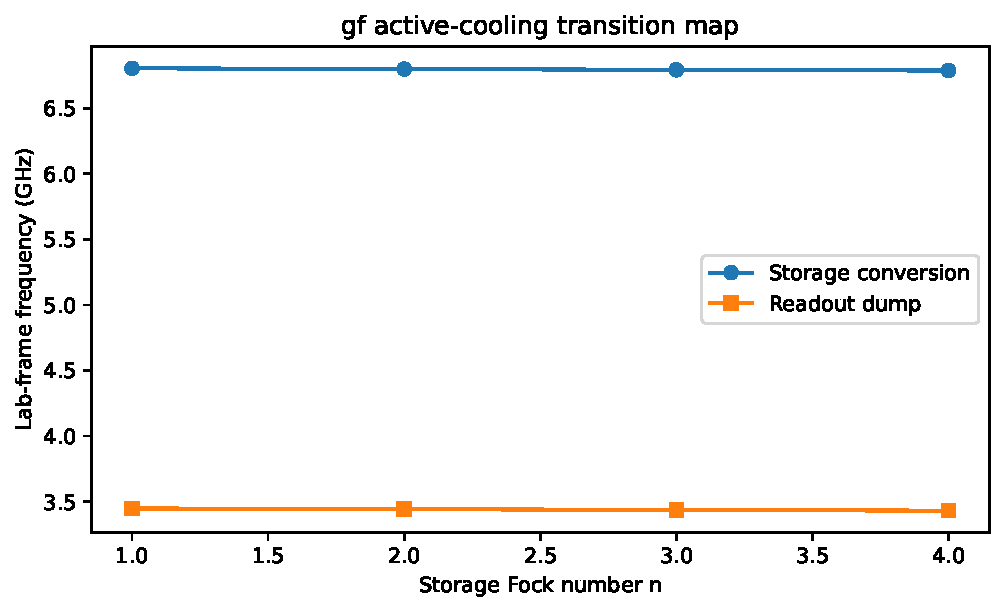
\includegraphics[width=\columnwidth]{../figures/transition_map.pdf}
\caption{Lab-frame transition map for the storage-conversion and readout-dump steps. Adjacent resolved lines are separated by \(5.680842~\si{\mega\hertz}\), so selectivity is set by bandwidth rather than large spectral gaps.}
\label{fig:transition_map}
\end{figure}

\subsection{Step A Pulse Design: Storage-to-Transmon Conversion}
The Step A scan screened seven waveform families over amplitude and duration grids. The key result is that the paper-motivated bump envelope is not merely a stylistic variation: it is the best practical Step A family for \(n_s=1\), \(3\), and \(4\), while a short square pulse wins only for \(n_s=2\). Figure~\ref{fig:family_comparison} shows the best transfer found for each family. The recommended Step A transfers are \(0.996051\), \(0.999421\), \(0.997767\), and \(0.996048\) for \(n_s=1,\ldots,4\).

The rejected families are also informative. The phase-modulated bump performs poorly for Step B, never exceeding about \(67.7\%\) transfer in the best readout-dump cases, but its Step A behavior is more nuanced: it can reach high transfer for \(n_s=1\) and \(4\), although only with much longer pulses such as \(\SI{160}{\nano\second}\) at \(n_s=1\) and \(\SI{80}{\nano\second}\) at \(n_s=4\). It is therefore not the best practical Step A choice even when its peak transfer is competitive. The derivative-corrected Gaussian triggers numerical stiffness in the present effective model and is therefore screened out as unreliable rather than promoted as a robust-control upgrade. These failures strengthen the conclusion that the best pulse is a genuinely shaped sideband ramp rather than an arbitrary smooth envelope.

\begin{figure}[t]
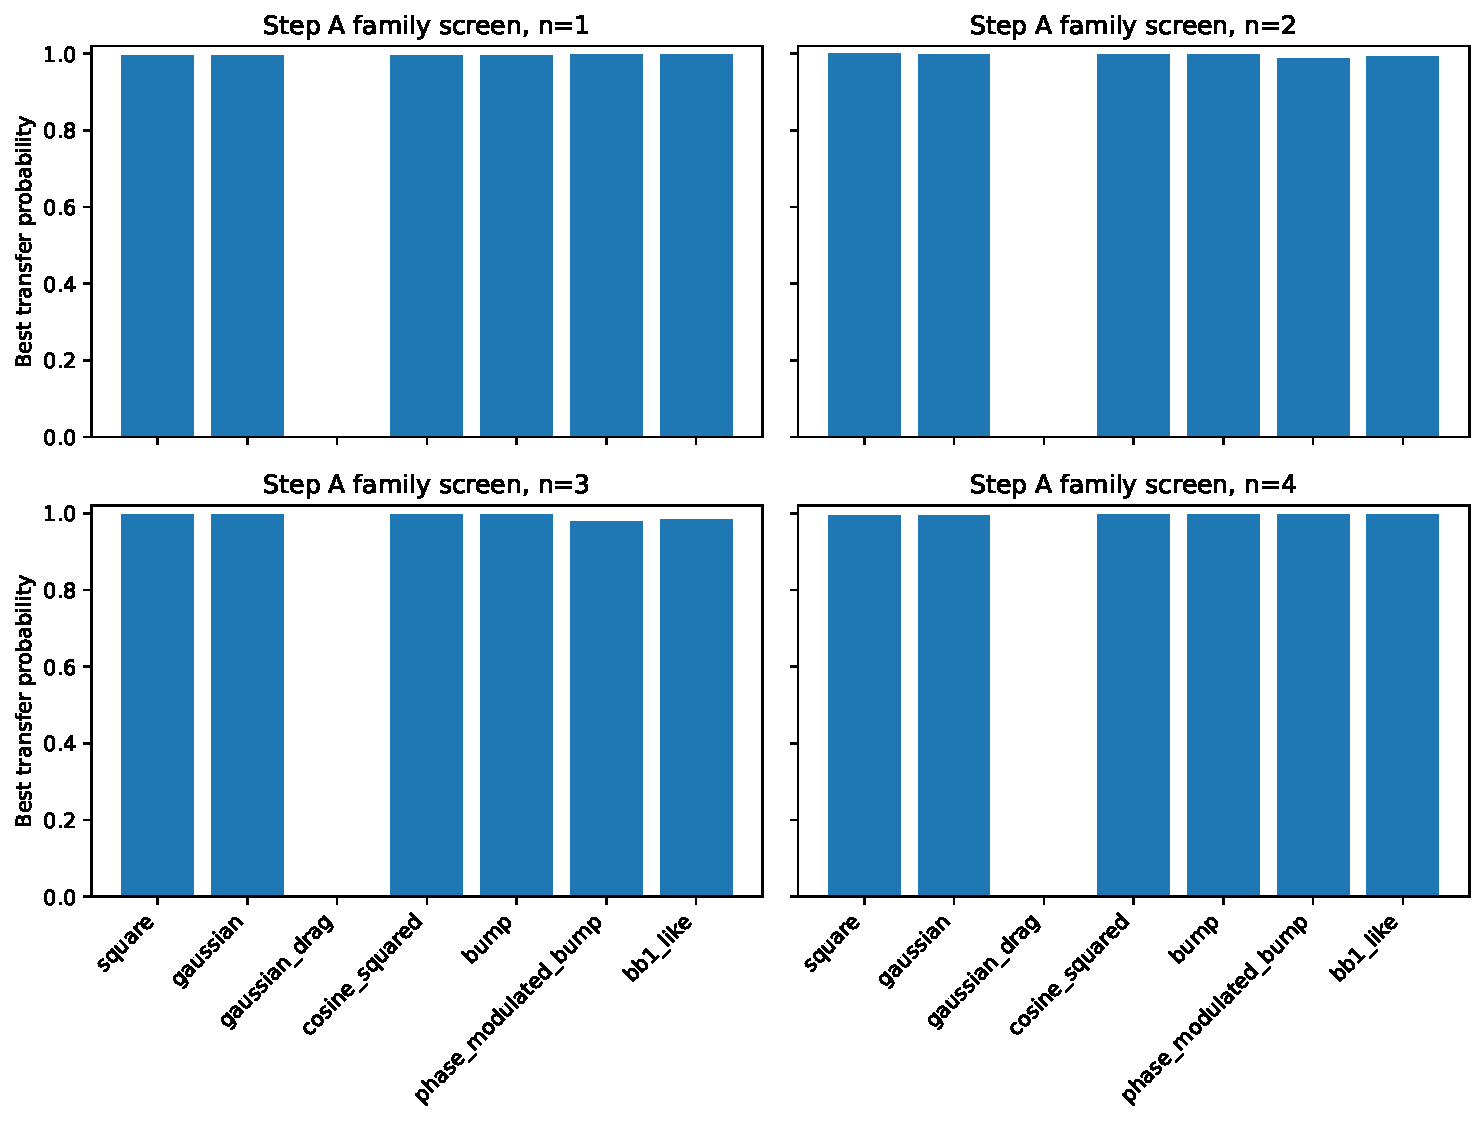
\includegraphics[width=\columnwidth]{../figures/storage_family_comparison.pdf}
\caption{Best closed-system transfer found for each Step A family and each \(n_s\). The bump family, motivated by the sideband literature, is the best practical Step A control for three of the four storage manifolds.}
\label{fig:family_comparison}
\end{figure}

The paper of Ref.~\onlinecite{huang2025fastsideband} also motivated a direct Stark-shift check. Figure~\ref{fig:calibration} shows the local detuning scans around each recommended pulse. Within the \(\pm\SI{2}{\mega\hertz}\) window tested here, every recommended Step A pulse is optimized at zero detuning relative to the static dressed frequency. This does not prove that hardware will show no Stark shift, because the present effective model does not include a microscopic pump Hamiltonian, but it does show that the recommended pulses are self-consistent within the simulator.

\begin{figure}[t]
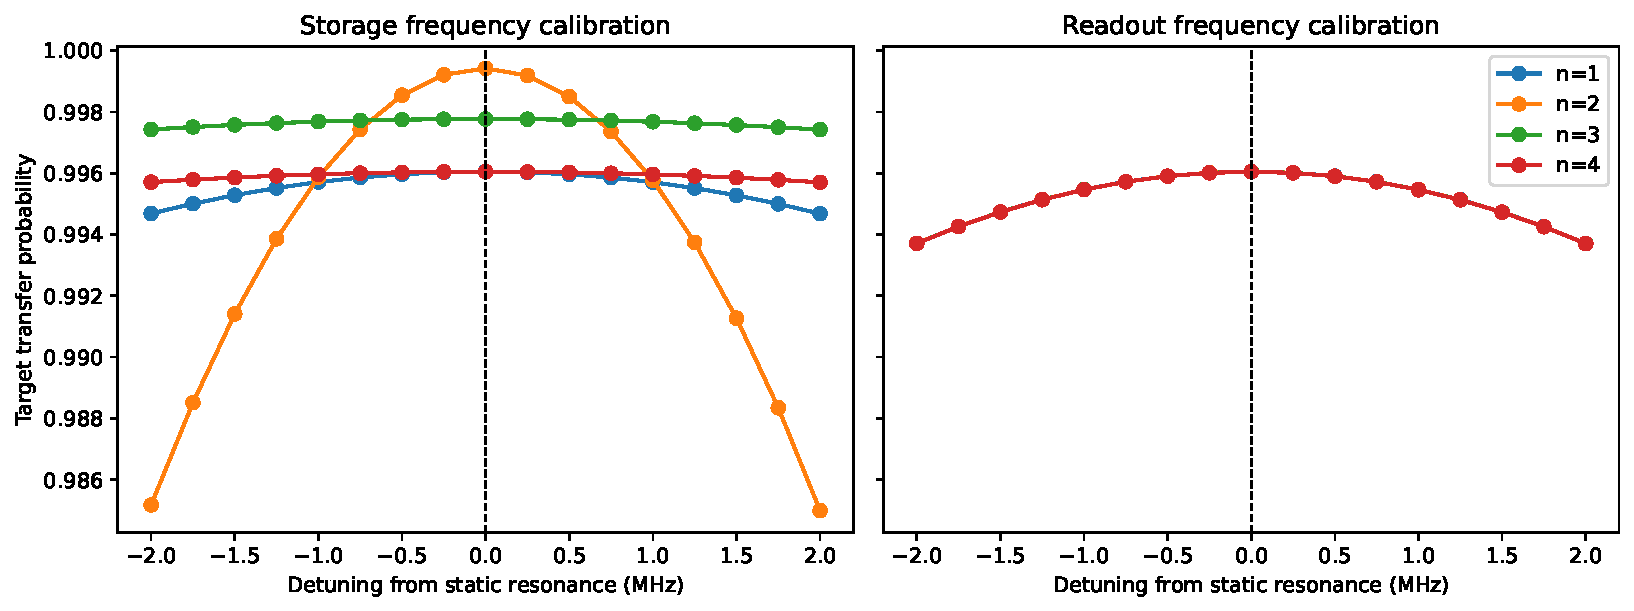
\includegraphics[width=\columnwidth]{../figures/frequency_calibration_curves.pdf}
\caption{Transfer versus local detuning for the recommended Step A and Step B pulses. In the effective model, every recommended pulse reaches its optimum at zero detuning within the \(\pm\SI{2}{\mega\hertz}\) scan window.}
\label{fig:calibration}
\end{figure}

\subsection{Step B Pulse Design: Transmon-to-Readout Dump}
The Step B transfer is simpler but no less important. A cosine-squared pulse with amplitude \(\SI{12}{\mega\hertz}\) and duration \(\SI{20}{\nano\second}\) is the best practical Step B family for every \(n_s\), with transfer probabilities of \(0.9960505\), \(0.9960498\), \(0.9960491\), and \(0.9960482\). The dominant closed-system leakage is simply incomplete transfer, that is, residual population left in \(\ket{f,0_r,n_s-1}\).

The physical interpretation is also clean. In contrast with Step A, Step B does not benefit from storage-ladder bosonic enhancement because the readout begins in vacuum. The readout transfer therefore stays near a fixed effective Rabi scale across \(n_s\), apart from the storage-dependent resonance shift that must be calibrated spectroscopically.

\subsection{Floquet Check and Strong-Drive Interpretation}
Reference~\onlinecite{huang2025fastsideband} emphasizes that strong sideband drives can produce substantial Stark shifts and qualitatively important Floquet dressing. The present study tested that possibility directly at the recommended operating points. Figure~\ref{fig:floquet} shows the resulting quasienergy splittings for the dominant target doublet.

\begin{figure}[H]
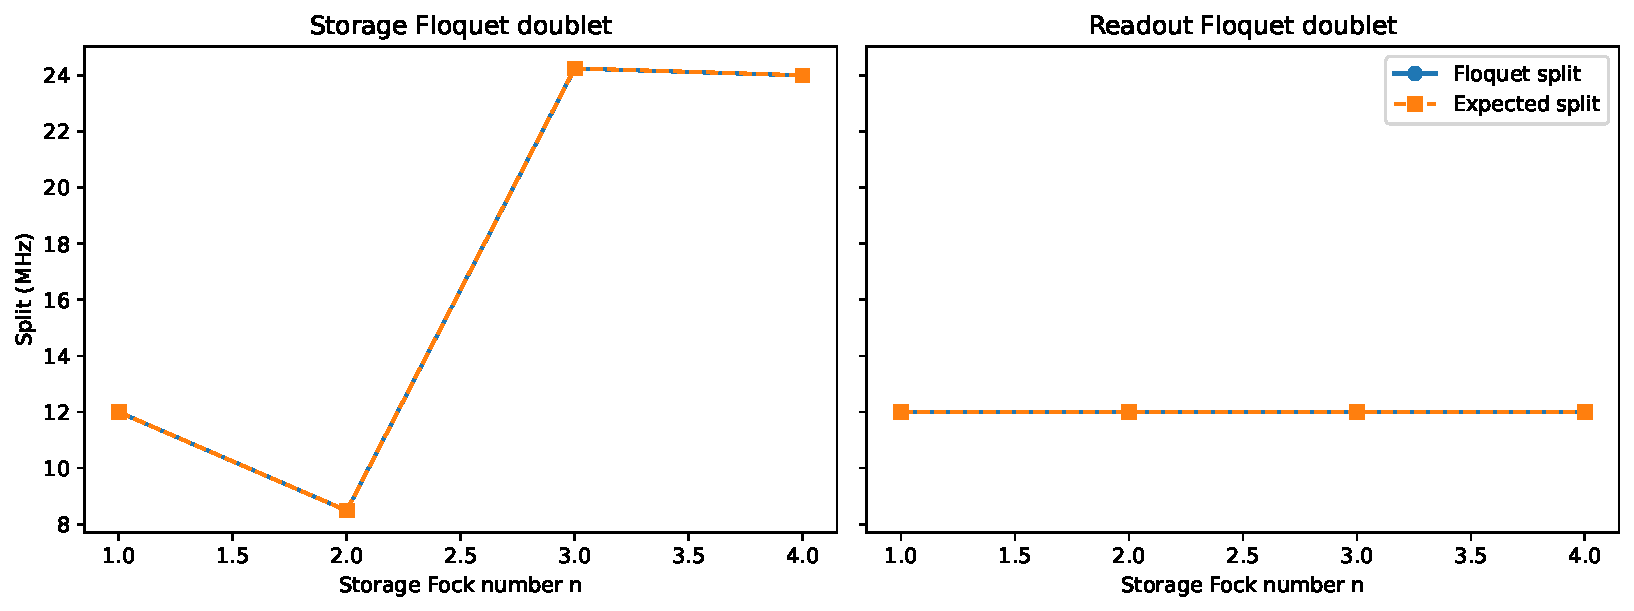
\includegraphics[width=\columnwidth]{../figures/floquet_doublet_splitting.pdf}
\caption{Floquet quasienergy split for the dominant target doublet at the recommended operating points. The storage sideband follows the expected \(\Omega\sqrt{n_s}\) scaling, while the readout sideband remains near the fixed \(\Omega\) scale.}
\label{fig:floquet}
\end{figure}

For Step A the quasienergy split tracks the expected bosonic enhancement very closely: \(\SI{11.999174}{\mega\hertz}\) for \(n_s=1\), \(\SI{8.485002}{\mega\hertz}\) for \(n_s=2\), \(\SI{24.242452}{\mega\hertz}\) for \(n_s=3\), and \(\SI{23.994182}{\mega\hertz}\) for \(n_s=4\). The corresponding deviations from the simple \(\Omega\sqrt{n_s}\) prediction are below \(\SI{6.3}{\kilo\hertz}\). For Step B the split stays near \(\SI{12}{\mega\hertz}\) for all \(n_s\), as expected from the absence of a bosonic factor. In every case the dominant target-doublet support is essentially unity.

The important caution is that every Floquet solve also reports noticeable weight on the truncation boundary. The Floquet results therefore support the target-doublet picture and the absence of a large unexpected shift, but they should not be over-interpreted as precision leakage estimates in the strong-drive regime.

\subsection{Full Cooling Primitive and Repeated Cycles}
The full cooling primitive combines a Step A pulse, a Step B pulse, and a passive wait of \(4/\kappa_r\). Figure~\ref{fig:primitive} shows the representative \(n_s=4\) trajectory. The population first moves into \(\ket{f,0_r,3}\), then into \(\ket{g,1_r,3}\), and finally decays toward \(\ket{g,0_r,3}\) during the readout ringdown.

\begin{figure}[H]
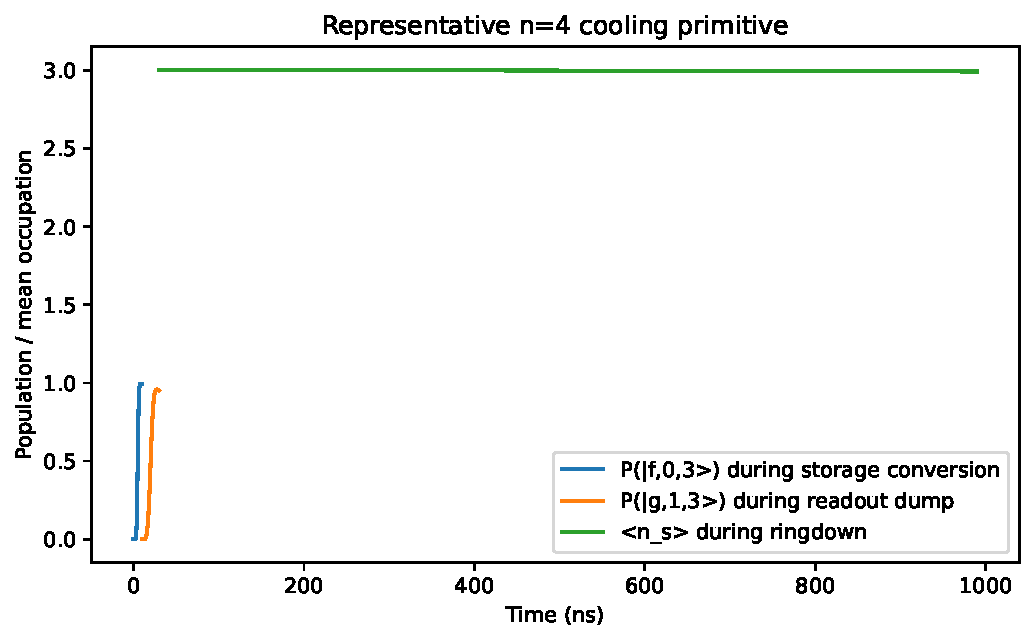
\includegraphics[width=\columnwidth]{../figures/cooling_primitive_trajectories.pdf}
\caption{Representative \(n_s=4\) cooling primitive. The storage pulse populates \(\ket{f,0_r,3}\), the dump pulse populates \(\ket{g,1_r,3}\), and the passive wait converts that readout excitation into irreversible storage cooling.}
\label{fig:primitive}
\end{figure}

\begin{table*}[t]
\caption{Single-cycle open-system cooling metrics. Success means final population in \(\ket{g,0_r,n_s-1}\). The residual transmon and readout columns separate incomplete dissipation from coherent transfer error.}
\label{tab:single_cycle}
\begin{tabular*}{\textwidth}{@{\extracolsep{\fill}}cccccc}
\toprule
\(n_s\) & Success & Final \(\avg{n_s}\) & Final transmon excitation & Final readout occupation & Dominant leakage \\
\midrule
1 & 0.9735 & 0.0039 & 0.0050 & 0.0176 & \(\ket{g,1_r,0}\) \\
2 & 0.9729 & 0.9965 & 0.0049 & 0.0177 & \(\ket{g,1_r,1}\) \\
3 & 0.9675 & 1.9943 & 0.0050 & 0.0176 & \(\ket{g,1_r,2}\) \\
4 & 0.9620 & 2.9921 & 0.0050 & 0.0176 & \(\ket{g,1_r,3}\) \\
\bottomrule
\end{tabular*}
\end{table*}

Table~\ref{tab:single_cycle} shows that the single-cycle success remains above \(96\%\) for all four storage manifolds. The dominant residual error after the full open-system cycle is not failure of Step A, but residual readout excitation left in \(\ket{g,1_r,n_s-1}\) because the passive wait is finite. Residual transmon excitation stays near \(0.5\%\), while the readout retains about \(1.76\times10^{-2}\) occupation after the fixed wait.

Repeated application matters more than a single idealized cycle because realistic storage states contain superpositions or mixtures of multiple \(n_s\) manifolds. Figure~\ref{fig:ladder} therefore applies the ladder sequentially to an initial basis state \(\ket{g,0_r,4}\), to a coherent-state test input with \(|\alpha|=1.1\), and to a thermal-like input with mean occupation near unity. The final mean storage occupations are \(0.07574\), \(0.03129\), and \(0.01251\), respectively.

\begin{figure}[H]
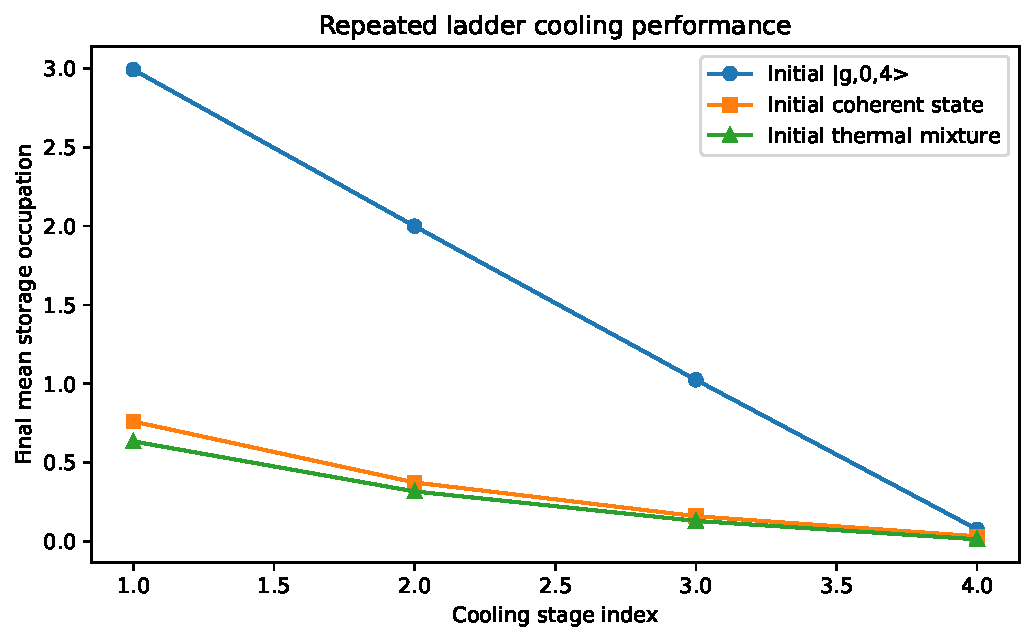
\includegraphics[width=\columnwidth]{../figures/cooling_per_cycle.pdf}
\caption{Repeated application of the cooling ladder to a basis state, a coherent state, and a thermal-like mixture. The protocol lowers the mean storage occupation strongly in all three cases, showing that it is a genuine cooling scheme rather than merely a one-step shelving process.}
\label{fig:ladder}
\end{figure}

These results answer the central physical question positively. In the effective model, the protocol of Eq.~\eqref{eq:cooling_cycle} is not just coherent population shuffling. It acts as a near-deterministic photon-subtraction primitive with a dissipative sink. The main degradation channels are spectral crowding, residual readout population, and transmon excitation that accumulates when several \(n_s\) manifolds are occupied simultaneously.

\section{Validation}
\label{sec:validation}

\subsection{Sanity Checks}
The first sanity check is analytic consistency. Equations~\eqref{eq:step_a_resonance} and~\eqref{eq:step_b_resonance} reproduce the numerically extracted rotating-frame resonances exactly to the printed precision for \(n_s=1,\ldots,4\). The second sanity check is the bosonic enhancement predicted by Eq.~\eqref{eq:step_a_projected}: the extracted storage-sideband matrix elements are \(1\), \(\sqrt{2}\), \(\sqrt{3}\), and \(2\), matching the expected ladder scaling exactly.

The third sanity check is a direct falsification of the most tempting wrong control picture. A resonant transmon \(g\leftrightarrow f\) carrier pulse populates \(\ket{f,0_r,n_s}\) with probability above \(0.99999994\) for every \(n_s\le4\), while leaving \(\ket{g,0_r,n_s-1}\) empty. The carrier therefore serves as a diagnostic but not as a cooling step.

\subsection{Convergence and Robustness}
The hardest case is the \(n_s=4\) open-system primitive. Table~\ref{tab:validation} shows that raising the transmon cutoff from 4 to 5 changes the success probability by \(2.79\times10^{-6}\), changing the storage cutoff from 7 to 6 or 8 changes it by at most \(4.35\times10^{-6}\), and changing the readout cutoff from 3 to 4 changes it by \(4.63\times10^{-5}\). Halving the timestep from \(0.25\) to \(\SI{0.125}{\nano\second}\) changes the success by \(9.22\times10^{-5}\), while doubling it to \(\SI{0.5}{\nano\second}\) changes the success by \(-3.39\times10^{-4}\). The study baseline is therefore numerically well converged for the present control-design questions.

\begin{table*}[t]
\caption{Validation summary for the hardest \(n_s=4\) cooling primitive.}
\label{tab:validation}
\begin{tabular*}{\textwidth}{@{\extracolsep{\fill}}lcccc}
\toprule
Case & \(\Delta f\) (kHz) & \(\Delta\) success & \(\Delta \avg{n_s}\) & Comment \\
\midrule
Analytic vs. numeric, \(n_s=1\) & 0.0 & --- & --- & exact to printed precision \\
Analytic vs. numeric, \(n_s=2\) & 0.0 & --- & --- & exact to printed precision \\
Analytic vs. numeric, \(n_s=3\) & 0.0 & --- & --- & exact to printed precision \\
Analytic vs. numeric, \(n_s=4\) & 0.0 & --- & --- & exact to printed precision \\
Transmon cutoff \(4\rightarrow5\) & 0.0 & \(+2.79\times10^{-6}\) & \(-3.44\times10^{-6}\) & negligible change \\
Storage cutoff \(7\rightarrow6\) & 0.0 & \(+4.35\times10^{-6}\) & \(-6.59\times10^{-7}\) & negligible change \\
Storage cutoff \(7\rightarrow8\) & 0.0 & \(+6.62\times10^{-7}\) & \(-2.31\times10^{-6}\) & negligible change \\
Readout cutoff \(3\rightarrow2\) & 0.0 & \(+4.22\times10^{-6}\) & \(+5.71\times10^{-6}\) & negligible change \\
Readout cutoff \(3\rightarrow4\) & 0.0 & \(+4.63\times10^{-5}\) & \(-4.21\times10^{-6}\) & still small \\
Timestep \(0.25\rightarrow\SI{0.125}{\nano\second}\) & 0.0 & \(+9.22\times10^{-5}\) & \(-8.64\times10^{-5}\) & finer-grid confirmation \\
Timestep \(0.25\rightarrow\SI{0.5}{\nano\second}\) & 0.0 & \(-3.39\times10^{-4}\) & \(+1.69\times10^{-4}\) & visibly less accurate \\
\bottomrule
\end{tabular*}
\end{table*}

Figure~\ref{fig:sensitivity} in Appendix~\ref{app:detailed} shows the local robustness maps for the recommended Step A pulses. Within a \(\pm\SI{1}{\mega\hertz}\), \(\pm10\%\) window around the selected pulse parameters, the transfer remains above \(95\%\) for all \(n_s\). That robustness is encouraging, but it must be interpreted together with the \(5.680842~\si{\mega\hertz}\) line spacing: moderate calibration drift is tolerable, yet strong spectral isolation should not be assumed.

\subsection{Literature Comparison}
The comparison to Ref.~\onlinecite{huang2025fastsideband} serves two purposes. The first is conceptual. That paper establishes that charge-driven sideband control can be fast, photon-number-resolved, and strongly influenced by bosonic enhancement, Stark shifts, and Floquet dressing. The second is methodological. It motivates calibrating each \(n_s\)-resolved transition separately and screening smooth ramps against square pulses.

The present results are consistent with those lessons while also clarifying the boundary of the local model. The bump family indeed emerges as the best Step A choice for most \(n_s\), supporting the paper's qualitative message that smooth ramps can outperform square pulses. The extracted Floquet doublet splittings track the expected \(\Omega\sqrt{n_s}\) scaling, which supports the same sideband-ladder interpretation. At the same time, the absence of a resolved detuning shift in Figure~\ref{fig:calibration} should not be read as a contradiction of the paper's Stark-shift observations; it reflects the fact that the present simulator uses effective sideband operators rather than a microscopic pump Hamiltonian.

\section{Discussion}
\label{sec:discussion}
The main physical conclusion is that the local device supports a viable storage-cooling ladder through \(n_s=4\), provided the protocol is implemented as a pair of effective sidebands plus readout decay rather than as a direct transmon carrier drive. The Step A resonance is storage-photon-number selective, bosonically enhanced, and fast enough to be useful. The Step B resonance is simpler, nearly \(n_s\)-independent in effective rate, and adequately selective when driven with a cosine-squared pulse.

The main experimental difficulty is spectral crowding. The \(n_s\)-resolved lines are only \(5.680842~\si{\mega\hertz}\) apart, so a strong broad-band pulse that works on a single basis state can become problematic for superpositions and mixtures. This is visible in the coherent-state ladder, where the first cycle leaves \(4.17\%\) transmon excitation. The experiment-facing recommendation is therefore conservative: use the frequency table of Table~\ref{tab:recommendations} as the initial spectroscopy map, calibrate each \(n_s\) separately, and verify broad-state performance before optimizing for minimum duration.

The minimum convincing experimental validation stack is:
\begin{enumerate}
\item perform number-resolved Step A spectroscopy near the frequencies in Table~\ref{tab:recommendations};
\item sweep the pulse duration at each resolved line to extract the effective \(\pi\)-time and confirm the \(\sqrt{n_s}\) rate trend;
\item calibrate the Step B dump transitions and verify readout ringdown after the fixed wait;
\item demonstrate one-cycle population transfer from \(\ket{g,0_r,n_s}\) to \(\ket{g,0_r,n_s-1}\) for each \(n_s\);
\item measure repeated-cycle suppression of the storage photon-number distribution;
\item only after those checks pass, perform higher-overhead diagnostics such as storage Wigner tomography.
\end{enumerate}

This sequence is intentionally modest. The present study already indicates that the decisive question is not whether the ladder can work in principle, but whether the experimental pump can realize the same effective sideband Hamiltonian with sufficient selectivity and without introducing a larger Stark shift than the effective model predicts.

\section{Conclusion}
The storage-cooling ladder
\(\ket{g,0_r,n_s}\rightarrow\ket{f,0_r,n_s-1}\rightarrow\ket{g,1_r,n_s-1}\rightarrow\ket{g,0_r,n_s-1}\)
is viable in the local device model for \(n_s\le4\). The required Step A frequencies lie between \(6.787\) and \(\SI{6.804}{\giga\hertz}\), the Step B frequencies lie between \(3.432\) and \(\SI{3.449}{\giga\hertz}\), and the nearest competing line is always \(5.680842~\si{\mega\hertz}\) away. The best practical Step A controls are bump pulses for \(n_s=1,3,4\) and a short square pulse for \(n_s=2\), while Step B is best served by a cosine-squared pulse for all four storage manifolds. The full open-system primitive achieves \(96\%\) to \(97\%\) single-cycle success and strongly suppresses the storage occupation under repeated application.

The study therefore supports experimental pursuit of the protocol, with one explicit caution: the present amplitudes and detuning conclusions are statements about an effective sideband model, not yet about a microscopic pump calibration. That distinction does not weaken the control-design result, but it does define the next step required before claiming hardware-ready implementation.

\section{Limitations and Future Work}
\label{sec:future}
The following items are the main remaining work packages, ordered by priority.

\begin{enumerate}
\item \textbf{[P1 | HIGH] Microscopic pump model.} The current framework validates effective-control feasibility but does not derive the sideband matrix element, Stark shift, or parasitic couplings from the nonlinear circuit and the experimental pump line.
\item \textbf{[P1 | HIGH] Instrument-level calibration bridge.} The effective \(\SI{6}{\mega\hertz}\) to \(\SI{14}{\mega\hertz}\) amplitudes reported here are not generator powers or AWG voltages. A hardware translation layer is still needed.
\item \textbf{[P2 | MEDIUM] Strong-drive leakage analysis beyond the target doublet.} The Floquet calculations reproduce the expected quasienergy splits but warn about truncation-boundary weight. A higher-confidence strong-drive model should extend the accessible Hilbert space or reduce the problem further.
\item \textbf{[P2 | MEDIUM] Readout reset optimization.} The passive \(4/\kappa_r\) wait leaves residual readout population near \(1.7\times10^{-2}\). Hardware may prefer a slightly longer wait or active readout reset.
\item \textbf{[P3 | LOW] Extension beyond \(n_s=4\).} The present study establishes the low-photon regime. Larger \(n_s\) would test how quickly spectral crowding becomes prohibitive.
\end{enumerate}

\bibliographystyle{apsrev4-2}
\bibliography{references}

\appendix

\section{Detailed Results and Data}
\label{app:detailed}
Figure~\ref{fig:heatmaps} gives the Step A heatmaps for the best family at each \(n_s\). Figure~\ref{fig:sensitivity} shows local robustness to detuning and amplitude error. Figure~\ref{fig:wigner} shows the final storage Wigner function for the coherent-state cooling test. Table~\ref{tab:carrier} records the direct-carrier diagnostic that confirms why a bare transmon \(g\leftrightarrow f\) pulse is not a cooling mechanism.

\begin{figure}[H]
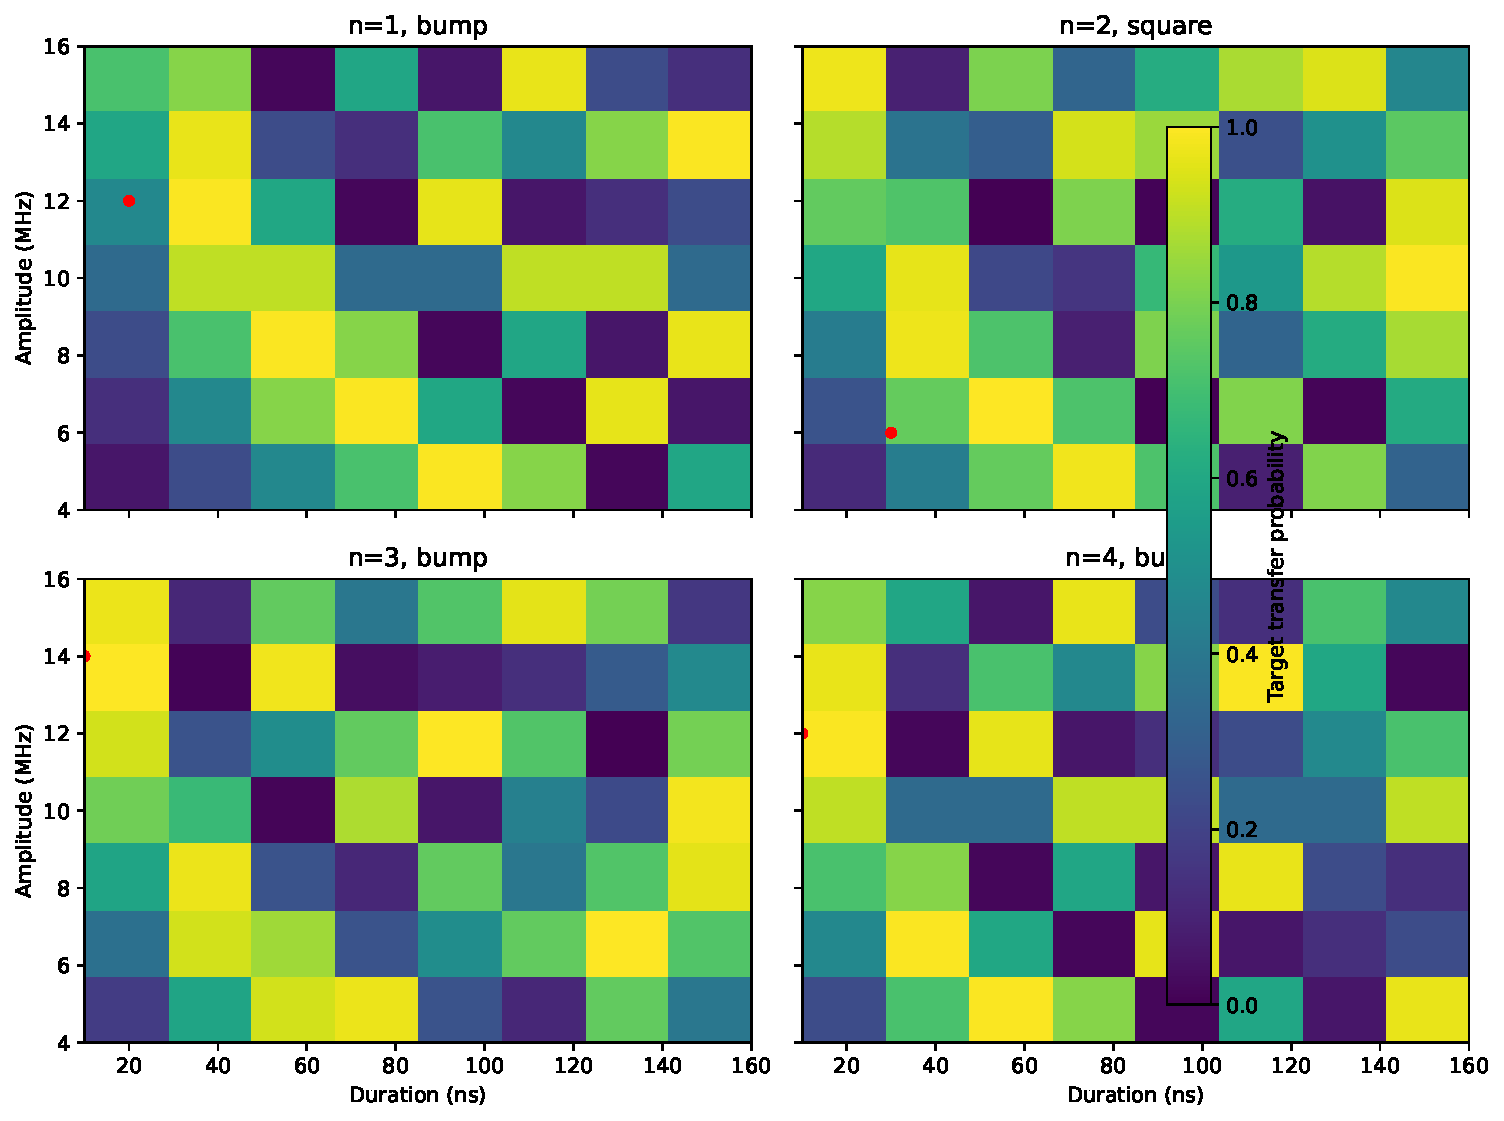
\includegraphics[width=\columnwidth]{../figures/storage_scan_heatmaps.pdf}
\caption{Step A transfer probability versus amplitude and duration for the best family at each \(n_s\). The high-fidelity lobes stay narrow enough to maintain number selectivity, but the allowed bandwidth is ultimately limited by the \(5.680842~\si{\mega\hertz}\) line spacing.}
\label{fig:heatmaps}
\end{figure}

\begin{figure}[H]
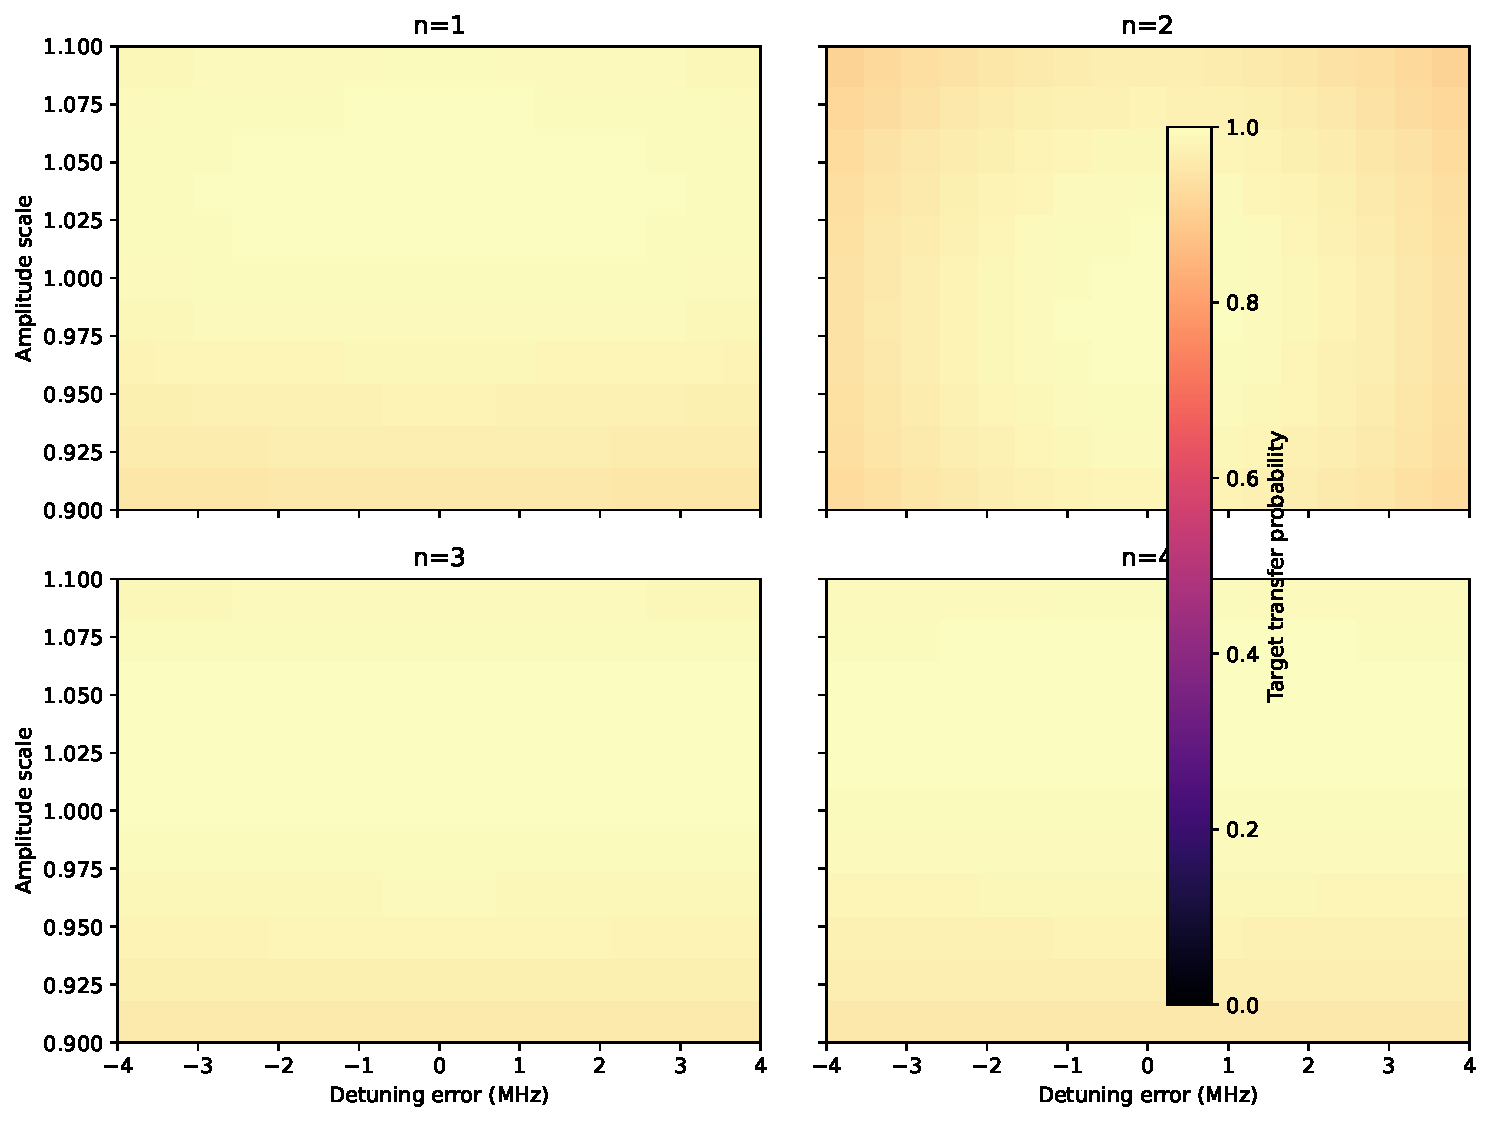
\includegraphics[width=\columnwidth]{../figures/sensitivity_heatmaps.pdf}
\caption{Local sensitivity of the recommended Step A pulses to detuning and amplitude error. All four recommended pulses remain above \(95\%\) transfer within a \(\pm\SI{1}{\mega\hertz}\), \(\pm10\%\) neighborhood.}
\label{fig:sensitivity}
\end{figure}

\begin{figure}[H]
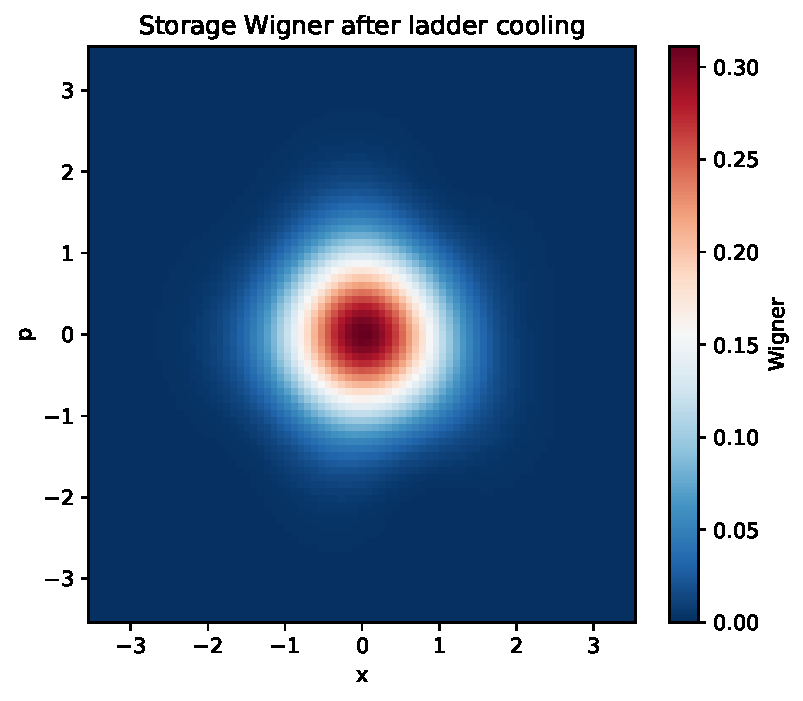
\includegraphics[width=\columnwidth]{../figures/coherent_final_wigner.pdf}
\caption{Storage Wigner function after applying the full four-step ladder to the coherent-state test input with \(|\alpha|=1.1\). The resulting distribution is concentrated near the vacuum region, consistent with the final mean occupation of \(0.03129\).}
\label{fig:wigner}
\end{figure}

\begin{table}[H]
\caption{Direct \(g\leftrightarrow f\) carrier diagnostic. The carrier shelves the transmon but does not remove a storage photon.}
\label{tab:carrier}
\begin{tabular}{cccc}
\toprule
\(n_s\) & \(P(\ket{f,0_r,n_s})\) & \(P(\ket{f,0_r,n_s-1})\) & \(P(\ket{g,0_r,n_s-1})\) \\
\midrule
1 & 0.999999957 & 0 & 0 \\
2 & 0.999999957 & 0 & 0 \\
3 & 0.999999946 & 0 & 0 \\
4 & 0.999999948 & 0 & 0 \\
\bottomrule
\end{tabular}
\end{table}

\clearpage
\section{Reproducibility}
\label{app:repro}
The study includes machine-readable artifacts, figures in both raster and vector form, and an executable notebook. The notebook loads saved results by default, exposes all tunable parameters in a single early cell, and provides commented recomputation cells for the expensive steps.

The recommended reproduction path is: load the notebook, inspect the saved spectroscopy and pulse data, and rerun the end-to-end study only if a different device configuration or truncation is needed. The saved artifacts are organized as follows.

\begin{description}
\item[\path{data/}] Machine-readable CSV and JSON summaries, including \path{frequency_table.csv}, \path{recommendation_table.csv}, \path{frequency_calibration_scan.csv}, \path{floquet_summary.csv}, \path{storage_scan_summary.csv}, \path{dump_scan_summary.csv}, \path{sensitivity_scan.csv}, \path{convergence_checks.csv}, and \path{study_results.json}.
\item[\path{artifacts/}] Supplemental JSON payloads used to build the report and notebook, including frequency analysis, pulse optimization, calibration scans, Floquet summaries, cooling primitive metrics, repeated-cycle protocols, carrier diagnostics, and validation digests.
\item[\path{figures/}] All publication figures in both PDF and PNG form, including the transition map, family comparison, calibration curves, Floquet splitting plot, cooling trajectories, repeated-cycle comparison, sensitivity maps, and the final Wigner snapshot.
\item[\path{scripts/reproducibility_notebook.ipynb}] Load-first interactive walkthrough that reproduces the study from the saved artifacts and exposes all tunable parameters in one early cell.
\item[\path{scripts/run_study.py}] End-to-end study driver; \path{scripts/convergence_checks.py} reruns the targeted convergence pass.
\end{description}

\end{document}
